\documentclass[utf8x, notes]{beamer}
%\usepackage[norsk]{babel}
\usepackage[utf8x]{inputenc}
\usepackage[T1]{fontenc}
\usepackage[absolute,overlay]{textpos}
\usepackage{tikz}
\usepackage{xparse}
\usepackage{xifthen}
\usetikzlibrary{calc, arrows,shapes, intersections, decorations.pathreplacing, decorations.text, decorations.pathmorphing, decorations.fractals}
\tikzstyle{every picture}+=[remember picture]
\tikzstyle{na} = [baseline=-.5ex]
\beamertemplatenavigationsymbolsempty

\definecolor{myGray}{rgb}{.5,.5,.5}
\setlength{\TPHorizModule}{\textwidth}
\setlength{\TPVertModule}{\textheight}
\newcommand{\myref}[1]{%
\begin{textblock}{1}[0,1](0.01,1.103)
\tiny{\color{myGray}{#1}}
\end{textblock}}

\mode<presentation>{
\usetheme{Frankfurt}
%\usecolortheme{dolphin}
% \usecolortheme{beaver}
\setbeamercovered{transparent}
}

\setbeamertemplate{footline}{}

\title{Molekylær modellering av oppsprekking i gasshydrater}
\author{Henrik Andersen Sveinsson}
\institute[Universitetet i Oslo] % (optional, but mostly needed)
{ Fysisk institutt\\
Det matematisk-naturvitenskapelige fakultet \\
Universitetet i Oslo
}
\date{8. mai 2015}

\AtBeginSection[]
{
  \begin{frame}<beamer>{Oversikt}
    \tableofcontents[currentsection]
  \end{frame}
}

\begin{document}

\begin{frame}
	\titlepage
\end{frame}

\begin{frame}
\frametitle{Oversikt}
\tableofcontents
\end{frame}

\section[Introduksjon]{Introduksjon og Bakgrunn}

\subsection{}
\begin{frame}
\frametitle{Hva er gasshydrater?}
\begin{columns}[cc]
\column{0.5\textwidth}
\begin{figure}
\includegraphics[width=0.8\textwidth]{../pictures/burning_hydrate.pdf}
\end{figure}

\column{0.5\textwidth}
\begin{itemize}
\item Et isliknende stoff som inneholder molekyler av stoffer som opptrer som gass under vanlige forhold.
\end{itemize}

\end{columns}
\myref{Figur: \textit{U.S. Geological Survey}}
\end{frame}

\subsection{}
\begin{frame}
\frametitle{Hvor finnes gasshydrater?}
\begin{figure}
\includegraphics[width=0.8\textwidth]{../pictures/hydrate_map_nice.pdf}
\end{figure}
\myref{Figur: \textit{The World Ocean Review, Marine Resources -- Opportunities and Risks, 2014}}
\end{frame}

\subsection{}
\begin{frame}
\frametitle{Bruksområder}

\end{frame}

\subsection{}
\begin{frame}
\frametitle{Risiko}
\begin{itemize}
\item \emph{the clathrate gun hypothesis}
\end{itemize}
\end{frame}


\section{Modellering}

\subsection{}
\begin{frame}
\frametitle{Molekylærdynamikk}

\end{frame}

\subsection{}
\begin{frame}
\frametitle{LAMMPS}
\begin{itemize}
\item Oppsett
\item Verifisering
\end{itemize}
\end{frame}

\subsection{}
\begin{frame}
\frametitle{TIP4P/ICE + UAM}
\end{frame}

\subsection{}
\begin{frame}
Simulert system
\end{frame}

\section{Resultater}

\subsection{}
\begin{frame}
\frametitle{Mekaniske egenskaper}
\end{frame}

\subsection{}
\begin{frame}{Måling av arealet til sprekkoverflaten}
\begin{columns}[c]
\column{0.5\textwidth}
Jeg bruker en Monte-Carlo-metode for å finne tilgjengelig overflate:
\begin{equation*}
A_{ss} = 2V\frac{n_s}{L}
\end{equation*}
\begin{table}
\begin{tabular}{ll}
$A_{ss}$ & overflatearealet \\
$V$ & volum av prøven \\
$n_s$ & antall krysninger vegg--tomrom \\
$L$ & total lengde av trukne linjestykker 
\end{tabular}
\end{table}

\column{0.5\textwidth}
	\begin{figure}
 	\centering
 	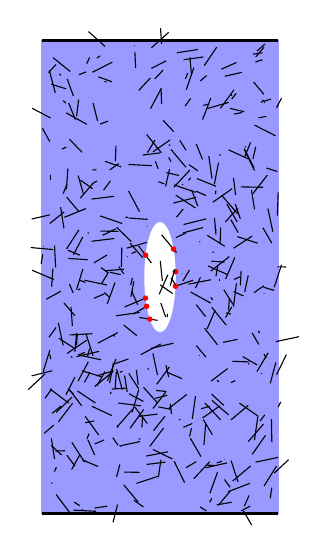
\begin{tikzpicture}
 		\filldraw[blue!40!white] (0, 0) rectangle (3, 6);
 		\draw[very thick] (0,0) -- (3, 0);
 		\draw[very thick] (0,6) -- (3, 6);
 		\fill[name path=myellipse, white] (1.5, 3) ellipse (0.2cm and 0.7cm);
 		\pgfmathsetseed{1138}
 		\foreach \x in {1,2,...,400} 
 		{
 			\pgfmathrandominteger{\a}{0}{300}
 			\pgfmathrandominteger{\b}{0}{600}
 			\pgfmathrandominteger{\c}{0}{359}
 			\pgfmathrandominteger{\d}{0}{180}
 			\pgfmathsetmacro{\length}{0.3*cos(\d)}
% 			%\def\length{\pgfmathresult}
 			\draw[name path=myline] (\a/100,\b/100) -- ++(\c:\length);
 			\def\n{0}
 			\fill [execute at begin node={\global\let\n=\n}, name intersections={of = myline and myellipse, total=\n}];
 			\pgfmathifthenelse{\n==1}{"\noexpand\fill [red] (intersection-1) circle (1pt)"}{"\noexpand\fill [blue] (2, 2) circle (0pt)"}
 			\pgfmathresult;
 		}
 	\end{tikzpicture}
	\end{figure}
	\end{columns}
\end{frame}

\subsection{}
\begin{frame}
\frametitle{Hovedresultat}
\begin{figure}
\includegraphics[height=0.95\textheight]{../figures/thesis/stress_area_lefm.pdf}
\end{figure}

\end{frame}


\section{Oppsummering og diskusjon}



\end{document}